\chapter{Processamento de Formulários}\label{cap:processamentoFormularios}
\epigraph{``\textit{O modo como você reúne, administra e usa a informação determina se vencerá ou perderá}''.}{Bill Gates}

\lettrine[lines=4, lhang=0.1, lraise=0, loversize=0.2, findent=0.1em]{\textcolor{corTema}{N}}{ESTE} Capítulo teremos como objetivos entender o funcionamento de formulários HTML e conseguirmos diferenciar os métodos do protocolo HTTP e como tratá-los.


\section{Introdução}

Neste Capítulo vamos começar a aprender a criar algo útil! No Capítulo~\ref{cap:javaParaWeb}, aprendemos as bases do desenvolvimento Web em Java, criamos alguns programas de brinquedo\footnote{Programa de brinquedo é todo programa criado para apresentar algum conceito e que, normalmente, não tem uma utilidade prática além da pedagógica.} para aplicar as técnicas que aprendemos e agora vamos aprender mais alguns detalhes, mas dessa vez nossos programas serão mais elaborados. Vamos começar?


\section{Formulários}

A forma tradicional de se desenvolver aplicações para Web que interajam com o servidor é utilizando os chamados formulários. Um formulário é composto normalmente por um conjunto de componentes que permitem que o usuário forneça dados para serem submetidos ao servidor. Quando esses dados são recebidos pelo servidor, algum componente da aplicação vai tratá-los, sendo que no nosso caso, esse componente vai ser implementado na forma de um Servlet.

Atualmente existem diversas técnicas para a criação de aplicações Web, sendo que, dependendo da técnica/tecnologia, a forma de submeter dados ao servidor é diferente. Uma dessas técnicas é o chamado \textit{Asynchronous JavaScript and XML} (AJAX) que hoje em dia é implementado de inúmeras formas. Neste livro aprenderemos sobre AJAX no Capítulo~\ref{cap:javaScript}.

Abra o NetBeans e crie um novo projeto Java Web. Dê o nome de ``PrimeiroFormulario'' (sem as aspas). Sempre que for criar um novo projeto, siga os passos descritos na Subseção~\ref{subsec:primeiroProjeto} do Capítulo~\ref{cap:javaParaWeb}. Com o projeto criado, vamos editar o \texttt{index.html}. Nele vamos alterar o título da página e criar nosso primeiro formulário, que será usado para preenchermos dados pessoais de um cliente. Veja na Listagem~\thechapter.\ref{listagem:projetos/capitulo02/parciais/indexInicio.html} como ficou o código. Não se esqueça de copiá-lo no seu \texttt{index.html}.

\htmlCode{Protótipo do formulário de dados do cliente (\texttt{index.html})}{projetos/capitulo02/parciais/indexInicio.html}

Copiou? Salve o arquivo e execute a aplicação. Você vai ter algo como o mostrado na Figura~\ref{fig:cap02PrimeiroFormulario}.

\FloatBarrier
\begin{figure}[!htbp]
    \centering
    \caption{Visualização do protótipo do formulário de dados do cliente}
    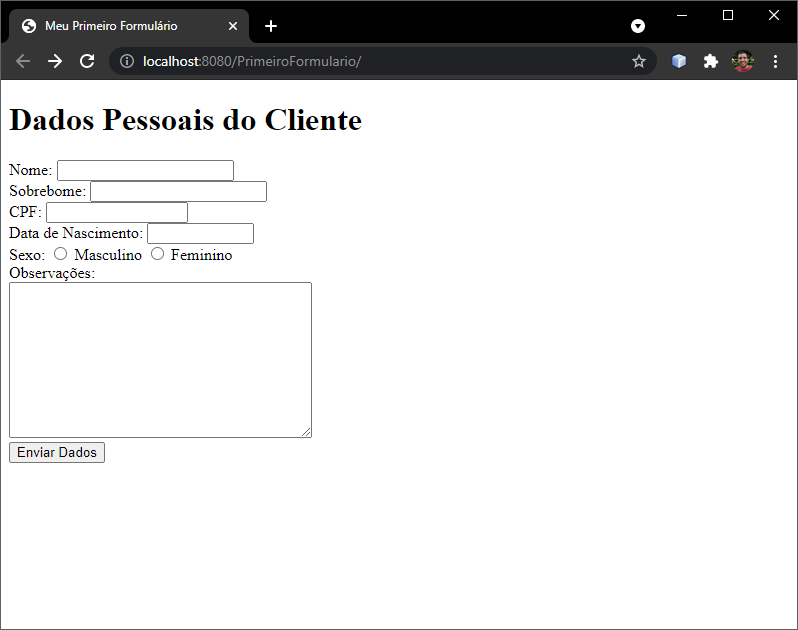
\includegraphics[scale=0.7]{imagens/cap02PrimeiroFormulario}
    \\\textbf{Fonte:} Elaborada pelo autor
    \label{fig:cap02PrimeiroFormulario}
\end{figure}
\FloatBarrier

Quanta coisa! O formulário não ficou uma obra prima, mas esse não é nosso objetivo agora. Precisamos entender o que cada \textit{tag} faz. Vamos agora analisar o código da Listagem~\thechapter.\ref{listagem:projetos/capitulo02/parciais/indexInicio.html} e entender o protótipo que fizemos. Irei detalhar apenas as \textit{tags} \inlineHTMLCode{<form>} e seus componentes, pois acredito que você já conheça as outras que foram utilizadas. Vamos lá então:

\begin{itemize}
    \item \textbf{Linha 13:} Nesta linha abrimos a \textit{tag} \inlineHTMLCode{<form>} que delimita um formulário HTML. Note que fechamos a \textit{tag} \inlineHTMLCode{<form>} na linha 43. Todas as \textit{tags} que forem inseridas entre \inlineHTMLCode{<form>} e \inlineHTMLCode{</form>} farão parte do formulário;
    
    \item \textbf{Linha 15:} Criamos um \textit{label} (tag \inlineHTMLCode{<label>}) com o conteúdo ``Nome: ''. A \textit{tag} \inlineHTMLCode{<label>} é usada para criar um rótulo. Ao invés de usar a \textit{tag} \inlineHTMLCode{<label>}, poderíamos simplesmente ter inserido o texto que queremos mostrar no formulário, mas como o texto que estamos utilizando tem o propósito de ser um rótulo para um campo do formulário, iremos utilizar essa tag para deixar nosso código mais organizado e inserir uma certa carga semântica no nosso código;
    
    \item \textbf{Linha 16:} Criamos um \textit{input} (campo de entrada) do tipo \textit{text} (texto) com tamanho de 20 colunas e com o nome de ``nome''. Dentre as \textit{tags} que representam componentes nos formulários, a \inlineHTMLCode{<input>} é uma delas. Existem vários tipos de \textit{inputs}, diferenciados pela propriedade \texttt{type}, e que vamos aprender aos poucos. A propriedade \texttt{size}, como você deve ter percebido, é utilizada para configurar a largura do campo de texto. A propriedade \texttt{name} é utilizada pelo navegador para identificar os dados do componente em questão no momento de enviar os dados para o servidor. Não entendeu a utilidade da propriedade \texttt{name}? Não se preocupe, logo vai fazer sentido;
    
    \item \textbf{Linha 17:} Usamos a \textit{tag} \inlineHTMLCode{<br/>} para pular uma linha;
    
    \item \textbf{Linhas 19 a 29:} Os próximos três campos (sobrenome, CPF e data de nascimento) são bem parecidos com o primeiro;
    
    \item \textbf{Linha 32:} Criamos um \textit{input} do tipo \textit{radio} (botão de rádio), com nome configurado como ``sexo'' e com o valor (\texttt{value}) configurado com ``M'';
    
    \item \textbf{Linha 33:} Idem à linha anterior, com a diferença que o valor é ``F''. Note que a propriedade name de ambos os radios é a mesma, pois eles representam o mesmo campo (sexo). Perceba que no navegador, se você selecionar um deles e depois clicar no outro, o que estava selecionado previamente deixa de ser selecionado. Se a propriedade \texttt{name} for diferente, eles serão considerados campos diferentes e então esse comportamento da seleção não existirá. Note ainda que você pode ``amarrar'' quantos radios você precisar;
    
    \item \textbf{Linha 38:} Nessa linha definimos uma área de texto. Esse componente, representado pela \textit{tag} \inlineHTMLCode{<textarea>} é utilizado, como o próprio nome já diz, para criar uma área de texto livre, onde o usuário poderá digitar uma quantidade arbitrária de texto. Note que para utilizar um \inlineHTMLCode{<textarea>} nós precisamos usar a \textit{tag} de fechamento (\inlineHTMLCode{</textarea>}), ao invés de fazer da forma que estamos fazendo com os \textit{inputs}. A novidade nesse componente são as propriedades \texttt{cols} e \texttt{rows}, que são usadas respectivamente para definir a quantidade de colunas e de linhas do componente;
    
    \item \textbf{Linha 41:} Por fim, nessa linha definimos um \textit{input} do tipo \textit{submit}, que é um botão que tem o comportamento padrão de, ao ser clicado, submeter (enviar) os dados do formulário para o servidor. Note que usamos a propriedade \texttt{value} para definir o texto do botão.
\end{itemize}

Agora que já conhecemos alguns dos componentes que podemos utilizar nos nossos formulários, mas você deve estar se perguntando: ``Tudo bem, o \textit{input} do tipo \textit{submit} é usado para enviar os dados do formulário para o servidor, mas onde eu digo ao \textit{submit} para onde os dados do formulário devem ser enviados?''. Vamos à resposta!

Eu tenho dito várias vezes que o componente que vai tratar os dados de um formulário na nossa aplicação é o Servlet não é mesmo? Então precisamos criar um Servlet que vai receber esses dados e então configurar o formulário para direcionar os dados inseridos nele para o Servlet apropriado.

Vamos criar o Servlet, mas agora iremos fazer de uma forma mais automática do que a que estamos fazendo desde que aprendemos a trabalhar com os Servlets. Na pasta de pacotes de código-fonte do projeto, crie um pacote chamado ``primeiroformulario.servlets'' (sem as aspas). Clique com o botão direito no pacote criado, escolha \destaque{\textit{New}} e procure pela opção \destaque{\textit{Servlet...}}. Se não encontrou, escolha a opção \destaque{\textit{Other...}}, selecione \destaque{\textit{Web}} na categoria, \destaque{\textit{Servlet}} no tipo de arquivo e clique em \destaque{\textit{Next >}}.

Preencha o campo \destaque{\textit{Class Name:}} com ``ProcessaDadosClienteServlet'' (sem as aspas) e clique em \destaque{\textit{Next >}}. Nesse passo, note que o assistente nos pede o nome do Servlet (\destaque{\textit{Servlet Name:}}) e o(s) padrão(ões) de URL (\destaque{\textit{URL Pattern(s):}}). Além disso, há a opção de inserir esses dados no descritor de implantação (\textit{deployment descriptor}), mas como estamos trabalhando com anotações para fazer o mapeamento do Servlet, essa opção deve ficar desmarcada. Falando sobre a anotação \inlineJavaCode{@WebServlet}, ao preenchermos esses campos, o NetBeans vai inserí-la para nós de forma automática! Deixe o campo \destaque{\textit{Servlet Name:}} com o valor padrão (que é o nome da classe) e preencha o campo \destaque{\textit{URL Pattern(s):}} com ``\texttt{/processaDadosCliente}'' (sem as aspas). Não iremos aprender sobre os parâmetros de inicialização (\textit{initialization parameters}) na nossa disciplina, mas nada impede que você aprenda para que eles servem, basta consultar a bibliografia recomendada nas referências bibliográficas do livro tudo bem? Tudo feito? Clique em \destaque{\textit{Finish}}.

Ao fazer isso, o nosso Servlet será criado e aberto no editor. Veja que a anotação \inlineJavaCode{@WebServlet} foi inserida apropriadamente no código da classe! Legal hein?

Note também que o NetBeans já implementou o esqueleto do Servlet para nós. O primeiro método implementado é o \inlineJavaCode{processRequest(...)}. Lembra-se dele? É nele que vamos inserir o código que queremos que o Servlet execute. Após o fechamento do bloco deste método, note que existe uma linha onde está escrito ``\textit{HttpServlet methods. Click on the + sign on the left to Edit the code.}''. Siga a sugestão da frase e clique no ``+''. O que apareceu? A implementação dos métodos \texttt{GET} e \texttt{POST}, sendo que dentro delas é chamado o \inlineJavaCode{processRequest(...)}! Viu só? Da mesma forma que fazíamos manualmente! Não iremos mexer ali, então você pode contrair novamente esta seção do código clicando no sinal de ``\texttt{–}''.

Note que além de implementar o esqueleto do nosso Servlet, o NetBeans também inseriu um trecho de código dentro do \inlineJavaCode{processRequest(...)}. O código que está inserido configura o que o Servlet gerará de resposta a quem o requisitou \linebreak(\inlineJavaCode{response.setContentType(...)}), obtém o fluxo de escrita do Servlet, escreve uma série de Strings que representam uma página HTML nesse fluxo e o fecha automaticamente, dado o uso do \textit{try with resources}. Você se lembra que já falei algumas vezes que não iremos implementar Servlets que geram código HTML? Então, vamos limpar esse método, tirando todo o código que foi inserido dentro dele. Vá no editor e apague o conteúdo entre as linhas 34 (\inlineJavaCode{response.setContentType(...)}) e 46 (\texttt{\}}), incluindo elas. Seu \inlineJavaCode{processRequest(...)} deve estar vazio agora.

Antes de escrevermos nosso código, vamos a mais um pouquinho de teoria. Você se lembra, lá no comecinho do Capítulo~\ref{cap:javaParaWeb}, que eu falei que o cliente manda uma requisição para o servidor e ele manda uma resposta? Nos Servlets, essa requisição e essa resposta são representadas respectivamente por objetos do tipo \texttt{HttpServletRequest} e \texttt{HttpServletResponse}. Note que os três métodos implementados nos nossos Servlets (\inlineJavaCode{processRequest(...)}, \inlineJavaCode{doGet(...)} e \inlineJavaCode{doPost(...)}) recebem dois parâmetros, sendo eles dos tipos que mencionei. Qual a conclusão que você chega então? Os dados enviados pelo cliente ao servidor estão dentro do objeto do tipo \texttt{HttpServletRequest}, que chamamos de \texttt{request} no nosso código e os dados que enviamos de volta ao cliente, ou a quem invocou o Servlet, devem ser inseridos no objeto do tipo \texttt{HttpServletResponse}, que demos o nome de \texttt{response}.

Sabendo disso, agora ficou fácil! Os dados do formulário de clientes que estamos construindo serão recebidos pelo nosso Servlet através do objeto apontado por \texttt{request}! Legal, mas ainda falta um detalhe... Não informamos ao navegador qual o destino dos dados do formulário! Vamos fazer isso agora. Volte no \texttt{index.html} e procure pela \textit{tag} \inlineHTMLCode{<form>} (a mesma que está na linha 13 da Listagem~\thechapter.\ref{listagem:projetos/capitulo02/parciais/indexInicio.html}). Para informarmos ao navegador qual o destino do dados do formulário, utilizamos a propriedade \texttt{action}, sendo que nesta propriedade, colocamos a URL do componente que deve tratar os dados do formulário. Mapeamos nosso Servlet usando o padrão \texttt{/processaDadosCliente} não foi? Então, qual será a URL do nosso Servlet? Resposta: \texttt{processaDadosCliente}. Vamos editar nossa \textit{tag} \inlineHTMLCode{<form>} então, configurando a propriedade \texttt{action} para a URL citada. Na Listagem~\thechapter.\ref{listagem:projetos/capitulo02/parciais/indexAction.html} você pode ver como ficou o código da \textit{tag} \inlineHTMLCode{<form>}. Note que não estou listando todo o arquivo.

\htmlCode{Configurando a propriedade \texttt{action} da \textit{tag} form (\texttt{index.html})}{projetos/capitulo02/parciais/indexAction.html}

Isso quer dizer que, quando clicarmos no botão ``Enviar Dados'' (que é um \textit{input} do tipo \texttt{submit}), os dados que estiverem nos componentes que estão dentro desse formulário serão enviados para o recurso \texttt{processaDadosCliente}, que é o endereço do nosso Servlet! Já alterou o arquivo? Salvou? Legal! Atualize a página, preencha os campos e clique no botão ``Enviar Dados''. O que aconteceu? Uma página em branco foi exibida não é? E na barra de endereços, o que apareceu? O endereço do Servlet mais um monte de ``coisas''! Os detalhes sobre isso nós iremos aprender na próxima seção, então não se preocupe por enquanto.

Você se lembra dos nossos primeiros exemplos? Acessávamos o endereço do Servlet, uma página em branco era exibida e duas Strings eram direcionadas para a saída do servidor, lembra? Quem fazia esse direcionamento era o Servlet, não era? Vamos fazer a mesma coisa com o nosso Servlet de dados dos clientes, mas mostraremos os dados que foram preenchidos nos formulários. Vamos lá então?

Volte ao Servlet, vamos implementar o método \inlineJavaCode{processRequest(...)}. Qual é mesmo o nome do parâmetro do método \inlineJavaCode{processRequest(...)} que armazena os dados enviados pelo cliente? É o \texttt{request} certo? Veja o código da Listagem~\thechapter.\ref{listagem:projetos/capitulo02/PrimeiroFormulario/src/java/primeiroformulario/servlets/ProcessaDadosClienteServlet.java}. Leia todos os comentário que fiz.

\javaCode{Implementação do método \texttt{processRequest} (\texttt{ProcessaDadosClienteServlet.java})}{projetos/capitulo02/PrimeiroFormulario/src/java/primeiroformulario/servlets/ProcessaDadosClienteServlet.java}

Copiou o código? Legal. Vamos entender o que está acontecendo. Primeiramente, na linha 31, para mantermos a consistência da codificação em que os dados da nossa aplicação estão trafegando entre as camadas, configuramos o \texttt{request} para processar seus dados usando o encoding \texttt{UTF-8}. Mais adiante no livro aprenderemos a criar um filtro que fará isso automaticamente para todos os nossos Servlets, mas por enquanto vamos fazer um a um, da forma que está no código.

Na linha 41 é declarada uma variável do tipo \texttt{String} com o nome de ``nome''. Essa variável é inicializada com o valor obtido ao se chamar o método\linebreak%
\inlineJavaCode{getParameter( String param )} de \texttt{request}. O parâmetro passado ao método \inlineJavaCode{getParameter( String param )}, que é uma \texttt{String}, é o nome que foi dado ao componente do formulário, que no caso foi ``nome''. Estude as linhas 42, 43, 44, 45 e 46 e tente fazer um paralelo com o formulário contido no \texttt{index.html}. Note que a String que é passada como parâmetro no método \inlineJavaCode{getParameter(...)} sempre reflete o nome dado ao componente do formulário através da propriedade \texttt{name}. Veja a linha 44. Declaramos uma variável chamada \texttt{dataNascimento} que é inicializada com o valor do parâmetro ``dataNasc'' (configurado no formulário).

O que fizemos até a linha 46 foi criar uma variável que vai receber o valor de cada componente do formulário. A partir da linha 48, até o final do método, direcionamos para a saída os dados que foram obtidos. Vamos testar? Salve o Servlet e execute o projeto (botão de ``play'', lembra?). Na página, preencha o formulário, clique em ``Enviar Dados'' e volte no NetBeans para ver o que aconteceu. Olhe na janela de saída! Lá estão os dados que você preencheu no formulário! Muito bem! Imagine agora se esse fosse um sistema real. Esses dados recebidos dentro do Servlet poderiam alimentar uma \textit{query} SQL para inserir esse cliente em um banco de dados! Legal não é?! A partir desse ponto, você já deve estar entendendo melhor o que está acontecendo, mas e aquele monte de coisas escritas no endereço do navegador depois de clicar em ``Enviar Dados''? Esse comportamento está intrinsecamente ligado ao tipo de método HTTP que estamos usando. Vamos para a próxima Seção, vou explicar isso lá.


\section{Métodos HTTP}

O protocolo HTTP que usamos em nossas aplicações Web, define uma série de métodos que podem ser usados para tratar diversos tipos de requisições. Na nossa vida, como desenvolvedores Web, iremos nos importar com vários desses métodos. Neste Capítulo trataremos os métodos \texttt{GET} e \texttt{POST}, que são os únicos que podem ser usados em formulários HTML. Sendo assim vamos a eles.

\begin{saibaMais}
    Quer conhecer os outros métodos HTTP como \texttt{HEAD}, \texttt{PUT}, \texttt{DELETE} etc.? Acesse este link: \url{https://developer.mozilla.org/pt-BR/docs/Web/HTTP/Methods}
\end{saibaMais}


\subsection{Método GET}

O método \texttt{GET} (\textit{to get} = obter) é usado principalmente para pedir ao servidor algum recurso, sendo que ele retornará os dados requisitados, caso existam, claro. Quando nós fazemos uma pesquisa no Google ou clicamos em um \textit{link}, estamos usando o método \texttt{GET}. Qualquer URL que colocamos na barra de endereço do nosso navegador é enviada ao servidor usando o método \texttt{GET}. Vamos fazer um teste. Entre na página do Google (\url{www.google.com}) e pesquise por ``métodos http'' (sem as aspas). Ao clicar em pesquisar, o resultado será mostrado no navegador. Note que no meu caso eu fiz a busca digitando diretamente na barra do navegador Chrome. Veja a barra de endereços. Haverá algo assim:

\destaque{\texttt{https://www.google.com/search?q=métodos+http\&oq=métodos+http\&aqs=chrome.....}}

Parece grego, mas não é! Vamos entender a URL. Estamos usando o protocolo HTTP, para acessar a máquina \texttt{www.google.com} e o recurso inicia em \texttt{search} e, a partir do ponto de interrogação, são codificados os parâmetros enviados na requisição do recurso:

\destaque{\texttt{q=métodos+http\&oq=métodos+http\&aqs=chrome.....}}

Dividindo esse resto da URL nos símbolos ``\&''. Vamos obter isso aqui:

\destaque{\texttt{q=métodos+http}}\\
\destaque{\texttt{oq=métodos+http}}\\
\destaque{\texttt{aqs=chrome.....}}\\
\destaque{\texttt{...}}

Note que a forma de cada pedaço da parte correspondente aos parâmetros enviados corresponde a é \texttt{x=y}, onde ``\texttt{x}'' é o nome de um parâmetro e ``\texttt{y}'' é o valor associado a ele. No nosso exemplo, o parâmetro ``\texttt{q}'' tem o valor ``métodos+http'' que no caso é a nossa consulta! Ou seja, o componente que trata as pesquisas do Google (\texttt{search}), entenderá que o parâmetro ``\texttt{q}'' vai conter o valor da pesquisa que estamos fazendo!

Execute novamente o nosso projeto, limpe todos os campos e preencha o campo ``Nome'' com ``Juca'' (sem as aspas) e o campo ``Sexo'' com Masculino e clique em ``Enviar Dados''. Veja a URL que foi obtida na barra de endereços:

\destaque{\texttt{http://localhost:8080/PrimeiroFormulario/processaDadosCliente?}}\\
\destaque{\texttt{nome=Juca\&\\sobrenome=\&cpf=\&dataNasc=\&sexo=M\&observacoes=}}

Veja o caminho do recurso!

\destaque{\texttt{processaDadosCliente?nome=Juca\&sobrenome=\&cpf=\&dataNasc=\&}}\\
\destaque{\texttt{sexo=M\&\\observacoes=}}

O que isso quer dizer que, no nosso caso, o Servlet mapeado no endereço ``processaDadosCliente'' receberá os parâmetros \texttt{nome}, \texttt{sobrenome}, \texttt{cpf}, \texttt{dataNasc}, \texttt{sexo} e \texttt{observacoes}, receberá os valores associados a ele para serem usados e deverá, de alguma forma, retornar o recurso associado a eles. O ponto de interrogação após o mapeamento do Servlet (\texttt{/processaDadosCliente}) indica que o que vem depois dele (do ponto de interrogação) são parâmetros HTTP. Cada parâmetro, como já vimos, está na forma \texttt{x=y}, onde ``\texttt{x}'' é o parâmetro e ``\texttt{y}'' é o valor, sendo que eles são separadas por ``\&''. Então temos: \texttt{nome} igual a ``Juca'', \texttt{sobrenome} igual a vazio, \texttt{cpf} igual a vazio, \texttt{dataNasc} igual a vazio, \texttt{sexo} igual a ``M'' e \texttt{observacoes} igual a vazio. A saída no NetBeans deve ter ficado assim:

\texttt{Dados do Cliente:|\#]}\\
\texttt{Nome: Juca|\#]}\\
\texttt{Sobrenome: |\#]}\\
\texttt{CPF: |\#]}\\
\texttt{Data de Nascimento: |\#]}\\
\texttt{Sexo: Masculino|\#]}\\
\texttt{Observações: |\#]}

Vamos mandar a requisição novamente para o NetBeans, só que agora modificando a URL ao invés de usar o formulário. Dê o sobrenome de ``Santos'' ao Juca e defina o CPF como 123456789. Preencheu a URL na barra de endereços? Tecle \texttt{<ENTER>} e veja o que aconteceu no NetBeans. A saída deve ter sido essa aqui:

\texttt{Dados do Cliente:|\#]}\\
\texttt{Nome: Juca|\#]}\\
\texttt{Sobrenome: Santos|\#]}\\
\texttt{CPF: 123456789|\#]}\\
\texttt{Data de Nascimento: |\#]}\\
\texttt{Sexo: Masculino|\#]}\\
\texttt{Observações: |\#]}

Então, basicamente, ao usarmos o método \texttt{GET}, indicamos que queremos algum recurso do servidor. Quando enviamos dados através do método GET, esses dados, na forma de parâmetros, são codificados na própria URL. O nosso formulário do \texttt{index.html} utiliza por padrão o método \texttt{GET}. Qualquer formulário usa por padrão o método GET, mas se quisermos mudar o método de envio do formulário, precisamos usar a propriedade \texttt{method} da \textit{tag} \inlineHTMLCode{<form>}. Ai você me pergunta: Porque usaríamos outro método? O \texttt{GET} já não funciona? E eu respondo: Sim, o \texttt{GET} funciona, mas imagine a seguinte situação: você vai armazenar os dados de um usuário de um sistema. Você vai mandar vários dados para o servidor, inclusive uma senha. O que acontece? A senha enviada vai aparecer na URL! Afinal, a senha é um campo do formulário! O ideal seria ninguém a ver correto? Outro problema. O tamanho de uma URL é fixo! Então não podemos mandar conteúdos de tamanho arbitrário, visto que iremos perder dados caso usemos o método \texttt{GET}! Imagine mandar um vídeo para publicação no YouTube! Então como fazemos? Método \texttt{POST}, ao resgate!


\subsection{Método POST}

O método \texttt{POST} (\textit{to post} = postar) é usado para enviar qualquer tipo de dados ao servidor o que, normalmente, acarretará em algum tipo de mudança no recurso requisitado ou mesmo no servidor. Ao contrário do método \texttt{GET}, ao usar o método \texttt{POST}, os parâmetros de um formulário não são inseridos na URL, mas sim no corpo da requisição. Sendo assim, a quantidade dos dados enviados usando o método \texttt{POST} pode ter qualquer tamanho, desde apenas um parâmetro, até arquivos de tamanhos variados. Você já enviou uma foto para o Facebook não enviou? Saiba que ela foi enviada usando o método \texttt{POST}.

Como eu já disse na seção anterior, por padrão, o navegador envia os dados de um formulário usando o método \texttt{GET}. Caso queiramos mudar esse comportamento, basta usar a propriedade \texttt{method} da \textit{tag} \inlineHTMLCode{<form>}. Vamos fazer isso? Vá ao NetBeans, abra o arquivo \texttt{index.html} caso não esteja aberto, procure pela \textit{tag} \inlineHTMLCode{<form>} e insira a propriedade \texttt{method}. Veja na Listagem~\thechapter.\ref{listagem:projetos/capitulo02/parciais/indexMetodo.html} como deve ficar.

\htmlCode{Usando o método \texttt{POST} para enviar a requisição para o Servlet (\texttt{index.html})}{projetos/capitulo02/parciais/indexMetodo.html}

Salve o arquivo e execute o projeto novamente. Preencha o formulário e clique em ``Enviar Dados''. Verifique a URL, pois agora os parâmetros não serão mais codificados nela. Verifique a saída no NetBeans para constatar que os dados continuam a ser enviados. Edite novamente o \texttt{index.html} e mude o método para \texttt{GET}. Teste novamente. Os parâmetros devem estar aparecendo novamente na URL não é? De novo, edite o \texttt{index.html}, volte para o método \texttt{POST} e teste de novo.

Muito bem! Estamos quase acabando. Tenho certeza que você deve estar entendendo tudo. Se não estiver, releia o que está com dúvida tudo bem? Vamos à nossa última Seção, onde trataremos de mais um pouquinho de teoria.



\subsection{Tratando Métodos HTTP}

Você deve lembrar que quando criamos um Servlet manualmente, nós criávamos três métodos, o \inlineJavaCode{processRequest(...)}, o \inlineJavaCode{doGet(...)} e o \inlineJavaCode{doPost(...)}. Quando criamos um Servlet usando o assistente do NetBeans, ele também cria uma estrutura parecida com a que a gente criava manualmente, além de já realizar o mapeamento do nosso Servlet usando a anotação \inlineJavaCode{@WebServlet}. Na seção anterior falamos dos métodos \texttt{GET} e \texttt{POST} do protocolo HTTP, que são os que nós usamos como desenvolvedores Web. Você já deve ter notado, e eu também já falei, que um Servlet deve implementar o método HTTP que ele deve tratar. A implementação de um método HTTP em um Servlet deve ser feita dentro de métodos que por padrão são nomeados \inlineJavaCode{doXXX(...)}, onde \texttt{XXX} deve ser trocado pelo nome do método HTTP em questão. Sendo assim, requisições usando o método \texttt{GET} são tratadas dentro do método \inlineJavaCode{doGet(...)} do Servlet. Requisições usando o método \texttt{POST} são tratadas dentro do método \inlineJavaCode{doPost(...)} do Servlet e assim por diante.

Note então que todos os Servlets que criamos até agora se comportam da mesma forma tanto para o método \texttt{GET} quanto para o método \texttt{POST}, pois sempre que a requisição chega no Servlet, o método apropriado é escolhido, entretanto, tanto o método \inlineJavaCode{doGet(...)}, quanto o método \inlineJavaCode{doPost(...)}, direcionam o fluxo de execução para o método \inlineJavaCode{processRequest(...)}!
 
Muito legal não é mesmo? Com isso fechamos este Capítulo. No próximo iremos aprender a trabalhar com dois recursos importantes da especificação das JSPs: \textit{Expression Language} (EL) e TagLibs. Após aprender essas duas funcionalidades, estaremos prontos para começar a criar nosso primeiro projeto que trabalha com banco de dados, mas antes disso ainda iremos formalizar e aprender algumas coisinhas. Ah, não se esqueça de praticar o que aprendemos até agora! Vamos ao resumo do Capítulo.


\section{Resumo}

Neste Capítulo demos um passo muito importante para a nossa vida como desenvolvedores Web, pois aprendemos a trabalhar com formulários e entendemos o funcionamento dos métodos GET e POST que fazem parte do protocolo HTTP. Como você já deve ter percebido, os formulários desempenham um papel importantíssimo nas aplicações Web. Tenho certeza que de agora em diante, sempre que você usar uma aplicação Web, você saberá como aquele formulário funciona. Para colocar em prática o que aprendemos, criamos um projeto Java Web no NetBeans e fizemos diversos testes.

\section{Exercícios}

\begin{exercicioSemArquivo}{}{}{}
    Qual a diferença entre os métodos \texttt{GET} e \texttt{POST}? Quando devemos utilizar um ou o outro?
\end{exercicioSemArquivo}

\section{Projetos}

\begin{projetoSemArquivo}{}{}{}
    Incremente o projeto que criamos durante o Capítulo inserindo mais alguns campos no formulário: email, logradouro, número, complemento, cidade, estado, CEP, se o cliente tem ou não filhos. Utilize apropriadamente os tipos de \textit{input} que aprendemos até agora.
\end{projetoSemArquivo}

\begin{projetoSemArquivo}{}{}{}
    Crie um novo projeto Java Web, com o nome de ``FormularioDVD'' (sem as aspas), que deve ter um formulário usado para enviar dados de um DVD. Um DVD, no nosso caso, deve ter: número, título, ator/atriz principal, ator/atriz coadjuvante, diretor/diretora e ano de lançamento. Para tratar o formulário, crie um Servlet usando o assistente do NetBeans. Esse Servlet deve obter os dados enviados através do formulário e imprimi-los na saída padrão usando \inlineJavaCode{System.out.println(...)}, como foi feito no exemplo construído durante este Capítulo. Esse formulário deve usar o método \texttt{POST}.
\end{projetoSemArquivo}

\begin{projetoSemArquivo}{}{}{}
    Crie um novo projeto Java Web, com o nome de ``FormularioProduto'' (sem as aspas), que deve ter um formulário usado para enviar dados de um Produto. Um Produto, no nosso caso, deve ter: código de barras, descrição, unidade de medida (unidade ou kg), quantidade por embalagem, fabricante (nome). Para tratar o formulário, crie um Servlet usando o assistente do NetBeans. Esse Servlet deve obter os dados enviados através do formulário e imprimi-los na saída padrão usando \inlineJavaCode{System.out.println(...)}, como foi feito no exemplo construído durante este Capítulo. Esse formulário deve usar o método \texttt{POST}.
\end{projetoSemArquivo}

\begin{projetoSemArquivo}{}{}{}
    Crie um novo projeto Java Web, com o nome de ``CalculadoraWeb'' (sem as aspas), que deve ter um formulário usado para atuar como uma calculadora. Nesse formulário, deve haver dois campos (``número 1'' e ``número 2'') e um conjunto de radios para representar a operação a ser realizada (adição, subtração, multiplicação e divisão). Para tratar o formulário, crie um Servlet usando o assistente do NetBeans. Esse Servlet deve obter os dados enviados através do formulário, executar a operação escolhida pelo usuário e imprimir o resultado na saída padrão usando \inlineJavaCode{System.out.println(...)}, como foi feito no exemplo construído durante este Capítulo. Esse formulário deve usar o método \texttt{GET}. Faça testes de envio dos dados usando apenas a URL gerada depois da primeira submissão.
\end{projetoSemArquivo}

\begin{projetoSemArquivo}{}{}{}
    Crie um novo projeto Java Web, com o nome de ``TamanhoString'' (sem as aspas), que deve ter um formulário com apenas um campo usado para enviar uma String de qualquer tamanho para um Servlet. Utilize uma \inlineHTMLCode{<textarea>} para o usuário poder inserir essa String no formulário. O Servlet deve obter a String enviada e imprimir a quantidade de caracteres da String na saída padrão usando \inlineJavaCode{System.out.println(...)}, como foi feito no exemplo construído durante este Capítulo. Qual método HTTP deve ser utilizado nessa situação? Justifique sua resposta.
\end{projetoSemArquivo}

\begin{projetoSemArquivo}{}{}{}
    Crie um novo projeto Java Web, com o nome de ``EhPrimo'' (sem as aspas), que deve ter um formulário usado para enviar um número inteiro para um Servlet, que por sua vez deve verificar se este número é primo. O resultado do teste deve ser impresso na saída padrão. Esse formulário deve usar o método \texttt{GET}.
\end{projetoSemArquivo}

\begin{projetoSemArquivo}{}{}{}
    Crie um novo projeto Java Web, com o nome de ``EquacaoSegundoGrau'' (sem as aspas), que deve ter um formulário usado para enviar os coeficientes de uma equação de segundo grau para um Servlet, que por sua vez deve calcular as raízes da equação em questão e imprimir essas raízes na saída padrão. As raízes de uma equação do segundo grau podem ser determinadas usando a fórmula de Bhaskara \url{http://pt.wikipedia.org/wiki/Bhaskara_II}. O Servlet deve verificar também se os coeficientes passados representam uma equação do segundo grau válida. Esse formulário deve usar o método \texttt{GET}.
\end{projetoSemArquivo}